\documentclass[12pt]{report}

\usepackage{paper} % Your custom style file
\addbibresource{Thesis.bib}

\begin{document}

% ===== TITLE PAGE =====
\pagenumbering{Alph}
\hypersetup{pageanchor=false}
\newcommand{\logopath}{figures/uhlogo.pdf} % Or just uhlogo.pdf if in the same directory
\newcommand{\thetitletext}{Construcción Incremental de Bases de Conocimiento Semi-estructuradas con Modelos de Lenguaje}
\newcommand{\theauthortext}{Carlos Mauricio Reyes Escudero}
\newcommand{\theadvisortext}{Dr.C Alejandro Piad Morffis}
\newcommand{\thedate}{Junio de 2025}
\newcommand{\theuniversitytext}{Universidad de La Habana}
\newcommand{\thefacultytext}{Facultad de Matemática y Computación}
\newcommand{\thedegreetext}{Trabajo de Diploma presentado en opción al título de \\ \textbf{Licenciado en Ciencia de la Computación}}

\begin{titlingpage}
\centering % Center all content within the page

% 1. University and Logo Block
{\large \theuniversitytext} \\
{\large \thefacultytext} \\ % Remove if not wanted
\vspace{0.5cm} % Space after text, before logo. Adjust if needed.
\includegraphics[width=3cm]{\logopath} % Keep logo width reasonable (e.g., 1.5cm to 2cm)

\vspace{2cm} % Space after logo, before title. Adjust this spacing.

% 2. Title
{\LARGE \bfseries \thetitletext \par} % Use \par for paragraph break after title
% Add manual spacing after title if needed, e.g., \vspace{1cm}
\vspace{2cm} % Space after title, before author. Adjust this spacing.

% 3. Author and Advisor
{\Large Autor: \theauthortext \par} % Author, use \par
\vspace{0.5cm} % Space between author and advisor
{\Large Tutor: \theadvisortext \par} % Advisor, use \par

% 4. Date (Optional, place it logically, e.g., after author/advisor or near bottom)
% \vspace{1cm} % Space before date
% {\large \thedate \par}

% Use \vfill to push the degree info to the bottom
\vfill

% 5. Degree Information
{\large \thedegreetext \par} % Degree Info, use \par
\vspace{1cm} % Add some space at the very bottom of the page

% 6. Date (Alternative position: At the very bottom)
{\large \thedate \par}
\vspace{1cm} % Add some space at the very bottom of the page
\end{titlingpage}
\cleardoublepage{}

% ===== FRONT MATTER =====
\pagenumbering{roman}
\setcounter{page}{1} % Reset counter for Roman numerals
\hypersetup{pageanchor=false}

% \thispagestyle{empty}% % No page number on dedication
   \vspace*{2.5cm} % Push down dedication text
\begin{flushright}
$\forall$ aquellos que aún buscan saber
\end{flushright}
%
\chapter*{Agradecimientos}
A tantas personas les debo, estar siquiera parado aquí hoy, ni hablar del tiempo para dedicarle a mis proyectos y aventuras, que no me alcanza el espacio para agradecer lo suficiente (y tampoco quiero que los profesores digan que hay más agradecimientos que tesis). Siento casi redundante agradecer a mi familia: si el universo es determinista, soy lo que soy por ellos, y si no lo es, lo soy gracias a ellos. Quiero agradecer a aquellos que han moldeado mi camino, poniendo a veces obstáculos y a veces dándome superpoderes; y a aquellos con quienes he tenido que saltar esos obstáculos o celebrar juntos las victorias. Perdonen la abstracción, pero pienso que en ella reside una gran habilidad del ser humano: saber de qué estamos hablando aunque solo dibujemos los bordes. Me deja pensando. Gracias.

% A tantas personas debo estar siquiera parado aquí hoy, ni hablar del tiempo para dedicarle a mis proyectos y aventuras, que no me alcanza el espacio para agradecer lo suficiente, y tampoco quiero que los profesores digan que hay más agradecimientos que tesis. Siento casi redundante agradecer a mi familia: si el universo es determinista, soy lo que soy por ellos, y si no lo es, lo soy gracias a ellos. Quiero agradecer a aquellos que han moldeado mi camino, poniendo a veces obstáculos y a veces dándome superpoderes; y a aquellos con quienes he tenido que saltar esos obstáculos o celebrar juntos las victorias. Perdonen la abstracción, pero pienso que en ella reside una gran habilidad del ser humano: saber de qué estamos hablando aunque solo dibujemos los bordes. Me deja pensando. Gracias.
\setcounter{page}{1} % Reset counter for Roman numerals
%\chapter*{Opinión del tutor}
asdasdasd
%\chapter*{Resumen}

La gestión del conocimiento personal (\textit{PKM}) enfrenta el desafío de integrar eficientemente nueva información. Esta tesis aborda este problema mediante el desarrollo de un sistema que automatiza la construcción incremental de bases de conocimiento semiestructuradas utilizando Grandes Modelos de Lenguaje (\textit{LLM}). Se presenta \textbf{lImporter}, un plugin para Obsidian.md implementado como un agente autónomo. La arquitectura del agente se basa en el paradigma \textit{ReAct} (Razonamiento y Acción), permitiéndole planificar y ejecutar tareas complejas. Utiliza \textit{function calling} para interactuar de forma fiable con la bóveda de notas del usuario y un sistema de optimización de contexto para analizar eficientemente el conocimiento existente y encontrar conexiones relevantes.

La eficacia y versatilidad del sistema se evaluaron a través de una serie de experimentos cualitativos. Estos demostraron la capacidad del agente para: (1) construir grafos de conocimiento estructurados a partir de texto no estructurado; (2) mantener y expandir una base de conocimiento existente, creando enlaces contextualmente apropiados; (3) adaptarse a flujos de trabajo de productividad como \textit{P.A.R.A}.; y (4) utilizar la base de notas como una memoria externa para resolver tareas iterativas, mostrando su potencial como herramienta computacionalmente universal. El trabajo concluye que la integración de agentes \textit{LLM} en sistemas de \textit{PKM} transforma estas herramientas de repositorios pasivos a colaboradores cognitivos activos, capaces de estructurar, conectar y generar nuevo conocimiento de manera autónoma.

\vspace{1cm}
\textbf{Palabras clave:} Gestión del Conocimiento Personal, Modelos de Lenguaje, Obsidian, Agentes Autónomos, ReAct, Grafos de Conocimiento.

\begin{otherlanguage}{english}    
\chapter*{Abstract}

Personal Knowledge Management (PKM) faces the challenge of efficiently integrating new information. This thesis addresses this problem by developing a system that automates the incremental construction of semi-structured knowledge bases using Large Language Models (LLMs). We introduce \textbf{lImporter}, an Obsidian.md plugin implemented as an autonomous agent. The agent's architecture is based on the \textit{ReAct} (Reasoning and Acting) paradigm, enabling it to plan and execute complex tasks. It leverages \textit{function calling} for reliable interaction with the user's note vault and employs a context optimization system to efficiently analyze existing knowledge and find relevant connections.

The system's effectiveness and versatility were evaluated through a series of qualitative experiments. These demonstrated the agent's ability to: (1) build structured knowledge graphs from unstructured text; (2) maintain and expand an existing knowledge base by creating contextually appropriate links; (3) adapt to productivity workflows such as P.A.R.A.; and (4) use the note vault as external memory to solve iterative tasks, showing its potential as a computationally universal tool. This work concludes that integrating LLM agents into PKM systems transforms these tools from passive repositories into active cognitive collaborators, capable of autonomously structuring, connecting, and generating new knowledge.

\vspace{1cm}
\textbf{Keywords:} Personal Knowledge Management, Large Language Models, Obsidian, Autonomous Agents, ReAct, Knowledge Graphs.

\end{otherlanguage}

% ===== LISTS =====
\cleardoublepage{}
\phantomsection{}
% \addcontentsline{toc}{chapter}{\contentsname}
\tableofcontents
\hypersetup{linkcolor=magenta, citecolor=green, urlcolor=magenta}
\cleardoublepage{}
\phantomsection{}
% \addcontentsline{toc}{chapter}{\listfigurename}
% \listoffigures

\cleardoublepage{}
\phantomsection{}
% \addcontentsline{toc}{chapter}{\listtablename}
% \listoftables

% ===== MAIN CONTENT =====
\cleardoublepage{}
\phantomsection{}
\pagenumbering{arabic}
\setcounter{page}{1} % Reset counter for Arabic numerals
\hypersetup{pageanchor=true}

\chapter{Introducción}
\label{chapter:introduccion}

% La gestión del conocimiento se ha convertido en una piedra angular en la era de la información, donde la capacidad de organizar, sintetizar y recuperar datos de manera eficiente es crucial para el desarrollo personal y profesional.
La sobrecarga de información en la actualidad plantea un desafío significativo para la productividad y el aprendizaje efectivo. En este contexto, la gestión del conocimiento personal emerge como una disciplina fundamental, no solo para académicos e investigadores, sino para cualquier individuo que busque optimizar su capacidad de aprendizaje y generación de ideas. Como señala \cite{ahrensHowTakeSmart2017}, una gestión eficaz de las notas y el conocimiento adquirido no solo facilita la escritura y el estudio, sino que transforma la manera en que se interactúa con la información, convirtiéndola en un activo dinámico y generador de nuevas perspectivas. El desarrollo de un \textit{segundo cerebro} \parencite{forteBuildingSecondBrain2022}, un sistema externo confiable para almacenar y conectar ideas, libera recursos cognitivos, permitiendo un enfoque más profundo en el pensamiento crítico y la creatividad.
El potencial de los Grandes Modelos de Lenguaje (\textit{LLM}) para revolucionar este campo es inmenso. Estas tecnologías ofrecen la posibilidad de automatizar y enriquecer la integración del conocimiento, asistiendo en la destilación de información, la identificación de conexiones y la generación de contenido relevante dentro de las bases de conocimiento personales. La automatización de estos procesos no solo promete un aumento en la eficiencia, sino también una democratización del acceso a metodologías avanzadas de gestión del conocimiento.

\section{Gestión del Conocimiento Personal}
\label{sec:pkm}
La Gestión del Conocimiento Personal (\textit{PKM}, por sus siglas en inglés) se define como el proceso mediante el cual un individuo recopila, clasifica, almacena, busca, recupera y comparte conocimiento en sus actividades diarias \parencite{grundspenkisAgentBasedApproach2007}. Esta disciplina es particularmente relevante para los denominados \textit{knowledge workers}, profesionales para quienes el conocimiento es su activo más valioso y que dedican una parte significativa de su tiempo a gestionar grandes cantidades de información. La PKM busca empoderar a estos individuos para que sean más efectivos en sus entornos personales y sociales.

\subsection{Toma de notas}
La toma de notas, lejos de ser un mero acto de transcripción, es una estrategia fundamental para mejorar el aprendizaje y la retención de información \parencite{jansenIntegrativeReviewCognitive2017}. Al tomar notas, el individuo no solo registra la esencia de la información, sino que también se involucra en un proceso activo de filtrado, organización y reestructuración del conocimiento.

Existen diversas metodologías para la toma de notas, que pueden clasificarse ampliamente en lineales y no lineales.
Las metodologías lineales implican registrar la información en el orden en que se recibe. Un ejemplo común es denominado \textit{outlining}, donde las notas y pensamientos se organizan de manera estructurada y lógica. Otra técnica lineal es el \textit{sentence method}, que consiste en anotar cada tema como una oración corta y simple, ideal para lecciones de ritmo rápido.

Las metodologías no lineales, por otro lado, utilizan la organización espacial y los diagramas para ensamblar la información. Entre estas se encuentra el \textit{charting}, útil para temas que pueden desglosarse en categorías. El \textit{mapping}, como los mapas mentales, organiza las ideas en una estructura de árbol a partir de un punto central. Las Notas Cornell, desarrolladas por Walter Pauk \parencite{paukHowStudyCollege2010}, dividen la página en secciones para notas, pistas y un resumen. Las \textit{guided notes} proporcionan un esquema predefinido con puntos clave faltantes que el estudiante completa.
Más allá de estas técnicas tradicionales, han surgido sistemas más sofisticados. El método \textit{Zettelkasten}, popularizado por Niklas Luhmann y descrito en detalle por \cite{ahrensHowTakeSmart2017}, se basa en la creación de notas atómicas interconectadas, formando una red de conocimiento que fomenta la generación de ideas y la escritura prolífica. Este sistema, aunque con raíces históricas, ha ganado nueva relevancia en la era digital. Por otro lado, el método PARA \textit{(Projects, Areas, Resources, Archives)}, propuesto por \cite{forteBuildingSecondBrain2022}, ofrece un marco para organizar la información digital en función de su accionabilidad, facilitando la gestión de proyectos y responsabilidades a largo plazo.

\subsection{Bases de Conocimiento Personal}
\label{subsec:pkb}
Una Base de Conocimiento Personal (\textit{PKB}) es una herramienta electrónica utilizada por un individuo para expresar, capturar y recuperar conocimiento personal. Se diferencia de una base de datos tradicional al contener material subjetivo y específico del propietario. El concepto de extender la memoria y las capacidades cognitivas del individuo mediante herramientas externas no es nuevo. Ya en 1945, Vannevar Bush imaginó el \textit{Memex} (de \textit{memory extension}), un dispositivo electromecánico en el que un individuo almacenaría todos sus libros, registros y comunicaciones, mecanizado de tal manera que pudiera ser consultado con gran velocidad y flexibilidad \parencite{bushWeMayThink1945}. Bush previó un futuro donde la sobrecarga de información requeriría nuevas formas de acceder y conectar el conocimiento acumulado.

La forma en que una PKB organiza el conocimiento se define por su modelo de datos. Estudios como los de Davies y colegas \parencite{daviesBuildingMemexSixty2005, daviesStillBuildingMemex2011} han analizado estos modelos en función de su marco estructural (cómo se interrelacionan los elementos), los elementos de conocimiento (las unidades básicas de información) y su esquema (el nivel de semántica formal). Un aspecto crucial destacado es la transclusión, la capacidad de ver el mismo elemento de conocimiento en múltiples contextos sin duplicación.

\paragraph{Grafos de Conocimiento Personal (\textit{PKG})}
Dentro de las PKB, los Grafos de Conocimiento Personal han ganado prominencia. Un PKG representa el conocimiento como una red de nodos interconectados, donde cada nodo es una pieza de información y las aristas representan las relaciones entre ellas, a menudo con visualizaciones gráficas que facilitan la exploración y el descubrimiento de conexiones \parencite{pyneMetaworkHowWe2022}.

\subsection{Sistemas Digitales de Toma de Notas}
\label{subsec:sistemas_digitales_toma_notas}
La visión del \textit{Memex} de Bush encuentra un eco contemporáneo en la plétora de sistemas digitales de toma de notas. Estos sistemas varían ampliamente en sus características y enfoques. Algunos, como \textit{Roam Research} y \textit{Logseq}, enfatizan los enlaces bidireccionales y la visualización gráfica, alineándose estrechamente con la idea de un \textit{PKG}. Otros, como \textit{Notion}, ofrecen una gran flexibilidad para crear bases de datos y vistas personalizadas, mientras que \textit{Evernote} y \textit{Google Keep} son populares por su simplicidad y accesibilidad multiplataforma. \textit{Microsoft OneNote} tiene casi todos los \textit{checks} en el articulo de la \textit{Wikipedia}. Alternativas de código abierto como \textit{Zettlr} y \textit{Joplin} también ofrecen robustas funcionalidades, a menudo con un enfoque en la privacidad y el control local de los datos. Herramientas más tradicionales como \textit{VimWiki} (para usuarios de \textit{Vim}) y \textit{OrgMode} (para \textit{Emacs}) ofrecen sistemas de toma de notas altamente personalizables y potentes para usuarios con conocimientos técnicos. \textit{Markor} y \textit{SimpleNote} se centran en la simplicidad y la edición \textit{Markdown}.

Entre estas herramientas, \textit{Obsidian.md} ha ganado una considerable popularidad para la escritura académica y la gestión del conocimiento personal. Siguiendo el modelo de datos de las \textit{PKB}, \textit{Obsidian} almacena las notas como archivos locales de texto plano en formato \textit{Markdown}, lo que garantiza la portabilidad y la longevidad de los datos. Su marco estructural se basa en un grafo de conocimiento, donde cada nota es un nodo y los enlaces bidireccionales permiten crear una red interconectada de información. Esto facilita la \textit{transclusión}, ya que una misma idea o nota puede ser referenciada y contextualizada desde múltiples puntos del grafo sin necesidad de duplicación. Los elementos de conocimiento son flexibles, desde conceptos simples hasta notas extensas. Obsidian también soporta un esquema enriquecido mediante el uso de metadatos (\textit{frontmatter}), etiquetas y la posibilidad de extender su funcionalidad mediante \textit{plugins}, como \textit{Dataview}, que permite realizar consultas complejas sobre las notas. Su vista de grafo visualiza las conexiones, ayudando a identificar relaciones y patrones emergentes.

\section{Grandes Modelos de Lenguaje}
\label{sec:llm}
Los Grandes Modelos de Lenguaje (\textit{LLM}) representan un avance transformador en el campo de la inteligencia artificial, con la capacidad de comprender, generar y manipular el lenguaje natural a niveles sin precedentes. Modelos como \textit{GPT-4} de \textit{OpenAI} \parencite{openaiGPT4TechnicalReport2024} y \textit{Gemini} de \textit{Google} \parencite{teamGeminiFamilyHighly2024} han demostrado habilidades notables en una amplia gama de tareas lingüísticas. En paralelo, la comunidad de código abierto ha respondido con modelos competitivos como \textit{DeepSeek} \parencite{deepseek-aiDeepSeekV3TechnicalReport2024}, \textit{Qwen} \parencite{baiQwenTechnicalReport2023} y \textit{LLaMa} \parencite{grattafioriLlama3Herd2024}, impulsando la innovación y la accesibilidad en este campo.

\subsection{Técnicas de \textit{Prompting}}
\label{subsec:prompting_techniques}
Para interactuar eficazmente con los LLM, se han desarrollado un sinfín de técnicas de \textit{prompting}. Inicialmente, se descubrió que proporcionar unos pocos ejemplos (\textit{few-shot learning}) mejoraba significativamente los resultados, apelando a la capacidad de generalización de los modelos sin necesidad de reentrenamiento \parencite{brownLanguageModelsAre2020}. Investigaciones posteriores han explorado qué partes de estos ejemplos son cruciales, sugiriendo que la estructura del texto o el formato pueden ser más importantes que la etiqueta correcta para que el modelo aprenda la tarea \parencite{minRethinkingRoleDemonstrations2022}.

Diversas estrategias se centran en guiar el comportamiento del modelo. El \textit{role-prompting} \parencite{kongBetterZeroShotReasoning2024}, que asigna un rol específico al LLM (e.g., actuar como un experto), y el \textit{style prompting} \parencite{luBoundingCapabilitiesLarge2023}, que especifica el estilo deseado, permiten adaptar la respuesta a necesidades concretas. Para mejorar la calidad en tareas complejas, se ha aprovechado la capacidad de los LLM para inducirlos a generar pasos intermedios de razonamiento, un enfoque conocido como \textit{cadena de pensamiento} (\textit{Chain-of-Thought}) \parencite{nyeShowYourWork2021, weiChainofThoughtPromptingElicits2023}. Este paradigma se ha extendido incluso a escenarios sin ejemplos (\textit{zero-shot CoT}), donde se instruye al modelo a \textit{pensar paso a paso} \parencite{kojimaLargeLanguageModels2023, wangPlanandSolvePromptingImproving2023}.

Otras técnicas se enfocan en la descomposición y la consistencia. El \textit{complexity-based prompting} aprovecha que respuestas más complejas a menudo correlacionan con una mayor probabilidad de acierto \parencite{fuComplexityBasedPromptingMultiStep2023}, mientras que la descomposición de problemas (\textit{least-to-most prompting}) resuelve sub-tareas más simples para integrar sus respuestas en la solución final \parencite{zhouLeasttoMostPromptingEnables2023}. La consistencia también se ha utilizado como criterio, generando múltiples respuestas y eligiendo la más frecuente (\textit{self-consistency}) \parencite{wangSelfConsistencyImprovesChain2023}. Para problemas que requieren planificación, estructuras como el \textit{Tree of Thoughts} y el \textit{Graph of Thoughts} permiten al LLM explorar diferentes caminos de razonamiento \parencite{yaoTreeThoughtsDeliberate2023, bestaGraphThoughtsSolving2024}.

Finalmente, se han desarrollado enfoques de auto-mejora y meta-razonamiento. Técnicas como \textit{Self-Ask} incitan al LLM a generar y responder preguntas de seguimiento para clarificar la tarea \parencite{pressMeasuringNarrowingCompositionality2023}, mientras que \textit{Self-Refine} establece un marco iterativo donde el modelo critica y mejora sus propias respuestas \parencite{madaanSelfRefineIterativeRefinement2023}. El \textit{step-back prompting} instruye al modelo a resolver primero una versión más abstracta del problema para simplificar la tarea \parencite{zhengTakeStepBack2024}. Otros enfoques exploran la inducción de un análisis previo del modo de proceder (\textit{meta-reasoning}) \parencite{gaoMetaReasoningLarge2024}, el uso de representaciones cognitivas como el \textit{Sketch of Thought} \parencite{aytesSketchofThoughtEfficientLLM2025} o la generación y evaluación iterativa de pasos de razonamiento (\textit{Cumulative Reasoning}) \parencite{zhangCumulativeReasoningLarge2025}.

\subsection{Optimización de Contexto}
\label{subsec:context_optimization}
A pesar de que los \textit{LLM} modernos poseen ventanas de contexto nominalmente muy grandes, su capacidad para utilizar eficazmente toda esa información es limitada, un fenómeno conocido como \textit{lost in the middle} \parencite{liuLostMiddleHow2024}. La optimización de contexto busca mitigar este problema presentando al modelo únicamente la información más relevante y densa para una tarea específica.

La principal estrategia para ello es la generación aumentada por recuperación (\textit{Retrieval-Augmented Generation} o \textit{RAG}), que combina la memoria paramétrica del \textit{LLM} con una memoria no paramétrica externa \parencite{lewisRetrievalAugmentedGenerationKnowledgeIntensive2021}. En lugar de procesar un documento extenso, un sistema \textit{RAG} primero recupera los fragmentos de texto más relevantes de una base de conocimientos (e.g., \textit{Wikipedia}) y luego los proporciona como contexto al LLM para que genere la respuesta final. La expansión de la ventana de contexto en modelos como \textit{Gemini 1.5} y \textit{Qwen2.5-1M} ha hecho que el aprendizaje con muchos ejemplos (\textit{many-shot in-context learning}) se vuelva una estrategia viable y potente, donde se pueden incluir numerosos ejemplos relevantes directamente en el \textit{prompt} \parencite{teamGemini15Unlocking2024, yangQwen251MTechnicalReport2025, agarwalManyShotInContextLearning2024}.

La efectividad de \textit{RAG} depende críticamente de la granularidad de la información recuperada. En lugar de recuperar pasajes de longitud fija, se ha demostrado que el uso de unidades más finas como las \textit{proposiciones} —unidades de texto atómicas y autocontenidas— mejora la densidad de la información relevante, reduce el ruido y aumenta el rendimiento en tareas posteriores \parencite{chenDenseRetrievalWhat2024}.

Más allá de la recuperación, han surgido marcos de compresión y razonamiento agentivo. \textbf{QwenLong-CPRS} es un sistema que, mediante instrucciones en lenguaje natural, comprime dinámicamente un contexto extenso en un resumen optimizado y específico para la consulta, actuando como un intermediario inteligente antes de pasar la información al \textit{LLM} final \parencite{shenQwenLongCPRS$infty$LLMsDynamic2025}. Por otro lado, la \textit{Cadena de Clarificaciones} (\textit{Chain-of-Clarifications}) propone un flujo de trabajo en el que el modelo se enseña a sí mismo generando preguntas de clarificación sobre la consulta original, recuperando evidencia para responderlas y refinando iterativamente su comprensión antes de dar la respuesta definitiva \parencite{zhuangSelfTaughtAgenticLong2025}. Finalmente, los \textit{Recitation-Augmented LLMs} se centran en mejorar la capacidad del modelo para recordar y citar fielmente la información del contexto proporcionado, ajustándolo para que aprenda a copiar explícitamente los segmentos relevantes, lo que mejora la fiabilidad de las respuestas basadas en el texto \parencite{sunRecitationAugmentedLanguageModels2023}.

\subsection{Agentes Basados en \textit{LLM}}
\label{subsec:agentes_llm}
El verdadero potencial de los \textit{LLMs} reside en su capacidad para actuar de forma autónoma y utilizar herramientas externas para superar sus limitaciones inherentes, como en cálculos matemáticos, razonamiento complejo o la verificación de hechos. A medida que los \textit{LLM} han mejorado, investigadores y empresas han explorado cómo permitirles interactuar con sistemas externos.

El sistema \textit{MRKL} (\textit{Modular Reasoning, Knowledge, and Language}) \parencite{karpasMRKLSystemsModular2022} es una de las formulaciones más simples de un agente, utilizando un LLM como \textit{router} para acceder a múltiples herramientas (e.g., obtener el clima o la fecha actual) y combinar la información para generar una respuesta final. Modelos como \textit{PAL (Program-aided Language Model)} \parencite{gaoPALProgramaidedLanguage2023} traducen problemas directamente a código ejecutable, mientras que \textit{ToRA (Tool-Integrated Reasoning Agent)} \parencite{gouToRAToolIntegratedReasoning2024} intercala pasos de código y razonamiento. El paradigma \textit{ReAct (Reasoning and Acting)} \parencite{yaoReActSynergizingReasoning2023} permite a los agentes generar un pensamiento, tomar una acción y recibir una observación, manteniendo un historial de estos pasos para informar decisiones futuras. \textit{Reflexion} \parencite{shinnReflexionLanguageAgents2023} extiende \textit{ReAct} incorporando retroalimentación lingüística para refinar el comportamiento del agente. (\textit{RAG}) se considera un sistema de agente cuando la propia recuperación se trata como una herramienta externa.

Para organizar la creciente diversidad de agentes y establecer un marco conceptual coherente, se han propuesto las \textit{Arquitecturas Cognitivas para Agentes de Lenguaje} (\textit{CoALA}, por sus siglas en inglés) \parencite{sumersCognitiveArchitecturesLanguage2024}. Inspirado en la ciencia cognitiva y la inteligencia artificial simbólica, \textit{CoALA} describe a los agentes de lenguaje en función de tres componentes clave: una memoria modular (de trabajo, episódica, semántica y procedimental), un espacio de acciones estructurado (acciones internas como razonar o aprender, y acciones externas para interactuar con el entorno) y un proceso de toma de decisiones generalizado. Este marco no solo permite clasificar y comparar los sistemas existentes, como \textit{ReAct} o \textit{Reflexion}, sino que también proporciona un plano para diseñar agentes futuros más capaces y estructurados, contextualizando los desarrollos actuales dentro de la historia más amplia de la IA.

\section{Extracción de Conocimiento y Enlaces}
\label{sec:extraccion_conocimiento_enlaces}
La extracción de conocimiento y la creación de enlaces entre piezas de información son tareas fundamentales en la construcción de bases de conocimiento robustas y útiles. Tradicionalmente, estos procesos han sido manuales y laboriosos, pero los avances recientes en \textit{LLMs} han abierto nuevas vías para su automatización y enriquecimiento.

\subsection{Extracción de Conocimiento}
La extracción de conocimiento, en el contexto de la gestión del conocimiento personal, implica identificar y capturar las ideas clave, entidades y relaciones presentes en diversas fuentes de información. Los \textit{LLM} han demostrado una notable capacidad para esta tarea, abordándola desde diversas perspectivas metodológicas.

Un enfoque fundamental es la \textit{extracción de conocimiento abierto}, que busca generar representaciones lógicas a partir de texto sin restricciones de dominio. Investigaciones pioneras como la de \parencite{vandurmeOpenKnowledgeExtraction2008} utilizan el procesamiento composicional del lenguaje para derivar proposiciones estructuradas, mientras que trabajos más recientes como \parencite{songOpenFactFactualityEnhanced2023} se centran en la veracidad y expresividad de los tripletes extraídos, utilizando marcos semánticos y enlaces a \textit{Wikidata} para garantizar la calidad. A escala industrial, \parencite{qianOpenDomainKnowledge2023} presenta un \textit{framework} para extraer conocimiento de la web abierta, abordando desafíos de volumen, variedad y veracidad.

Para estructurar este proceso, se han propuesto diversos \textit{frameworks} y \textit{pipelines} basados en \textit{LLM}. El trabajo de \parencite{zhangExtractDefineCanonicalize2024} introduce un marco de tres fases (Extraer-Definir-Canonizar) que realiza una extracción abierta seguida de una definición y canonización de esquemas \textit{post-hoc}, permitiendo una gran flexibilidad. De manera similar, \parencite{kommineniHumanExpertsMachines2024} propone un \textit{pipeline} semi-automatizado que abarca todo el proceso de construcción de grafos de conocimiento, desde la generación de preguntas de competencia (\textit{CQs}) hasta la creación de la ontología y su poblamiento, utilizando un '\textit{LLM} juez' para la evaluación. Un paradigma innovador es el de \parencite{liKnowCoderCodingStructured2024}, que representa los esquemas de conocimiento como clases de Python, un formato que los \textit{LLM} comprenden de forma nativa, y emplea un aprendizaje en dos fases para la comprensión y seguimiento del esquema. Por otro lado, \parencite{luoOneKEDockerizedSchemaGuided2025} diseña un sistema multi-agente (\textit{Schema, Extraction, Reflection}) para guiar la extracción de conocimiento en diversos dominios y formatos de datos.

La aplicación de estas técnicas a dominios específicos y la extracción guiada es otra área clave. Para el dominio clínico, \parencite{liAutomatedClinicalData2024} utiliza \textit{LLM} condicionados con conocimiento externo mediante aprendizaje en contexto (\textit{in-context learning}) para extraer información de informes médicos. Para garantizar la coherencia con bases de conocimiento existentes, enfoques como los de \parencite{fengOntologygroundedAutomaticKnowledge2024} y \parencite{mccuskerLOKELinkedOpen2023} utilizan ontologías preexistentes (como la de \textit{Wikidata}) para guiar y fundamentar el proceso de extracción del \textit{LLM}. Finalmente, la interacción con el usuario se explora en \parencite{abolhasaniLeveragingLLMAutomated2024}, que presenta un \textit{pipeline} interactivo guiado por un algoritmo adaptativo de Cadena de Pensamiento (\textit{CoT}) para alinear la extracción de ontologías con los requisitos del usuario.

\subsection{Creación de Enlaces}
La creación de enlaces se refiere al establecimiento de conexiones significativas entre las piezas de conocimiento extraídas. Los \textit{LLM} no solo extraen, sino que también pueden inferir y predecir estas relaciones.

Un paradigma dominante consiste en utilizar los \textit{LLM} para la predicción de enlaces como una tarea de inferencia. En este sentido, \parencite{shuKnowledgeGraphLarge2024} convierte la estructura del grafo en \textit{prompts} de lenguaje natural para afinar \textit{LLM} en la tarea de predicción de enlaces multi-salto. De forma similar, \parencite{heLinkGPTTeachingLarge2024} entrena un \textit{LLM} de extremo a extremo que integra información estructural pareada mediante un ajuste de instrucciones en dos etapas. Para abordar la escalabilidad en grafos de gran tamaño, \parencite{biLPNLScalableLink2024} propone un \textit{pipeline} de muestreo en dos etapas y una estrategia de 'divide y vencerás' para gestionar la sobrecarga de información en los \textit{prompts}.

Una estrategia diferente consiste en la creación de enlaces sin supervisión o con pocos ejemplos. El trabajo de \parencite{cartaIterativeZeroShotLLM2023} destaca en este aspecto, utilizando un \textit{pipeline} de \textit{prompting} iterativo en modo \textit{zero-shot}, que no requiere ejemplos ni recursos externos para construir el grafo de conocimiento.

Finalmente, otra línea de investigación utiliza los \textit{LLM} como enriquecedores de características para modelos existentes. En lugar de predecir el enlace directamente, \parencite{parkEnhancingFutureLink2024} emplea un \textit{LLM} para generar descripciones ricas de los nodos, que luego se utilizan como características iniciales para mejorar el rendimiento de los modelos de Redes Neuronales de Grafo (\textit{GNN}) en la predicción de enlaces, especialmente en escenarios de arranque en frío (\textit{cold-start}).

La combinación de estas dos capacidades —extracción y enlace— tiene el potencial de transformar la construcción de bases de conocimiento. Trabajos como los de \parencite{zhuLLMsKnowledgeGraph2024} y \parencite{machadoLLMStoreLeveraging2024} exploran las capacidades generales de los \textit{LLM} para estas tareas, el primero concluyendo que son mejores asistentes de inferencia que extractores, y el segundo implementando un \textit{LLM} como un 'almacén' de conocimiento dinámico que sintetiza respuestas estructuradas al momento de la consulta. La investigación continúa abordando desafíos como la interpretabilidad, la escalabilidad y la superación de las limitaciones inherentes de los \textit{LLM} mediante arquitecturas de agentes y la integración de herramientas externas.

\section{\textit{LLM} en Aplicaciones de Toma de Notas}
\label{sec:integracion_llm_pkm}
Los avances en los \textit{LLMs} han catalizado una diversidad de herramientas para automatizar y enriquecer la toma de notas y la gestión del conocimiento personal (\textit{PKM}). Estas varían desde aplicaciones web hasta \textit{plugins} para plataformas consolidadas, enfocándose en distintos casos de uso.

Un área prominente es la \textit{asistencia conversacional y la respuesta a preguntas contextualizadas}. En \textit{Logseq}, \textit{plugins} como \textit{Logseq Copilot} permiten interactuar con la IA, indexando las notas del usuario para ofrecer respuestas basadas en el propio conocimiento. En \textit{Obsidian.md}, herramientas como \textit{BMO Chatbot for Obsidian} y \textit{ChatGPT MD} ofrecen interfaces de chat versátiles, conectándose a servicios en la nube y \textit{LLMs} locales, y permitiendo referenciar la nota actual o notas enlazadas en las conversaciones. \textit{Caret Obsidian Plugin} extiende esta funcionalidad al \textit{Canvas} para un chat no lineal. \textit{Notion AI} también integra de forma nativa la capacidad de responder preguntas sobre el espacio de trabajo.

La \textit{generación y mejora de contenido} es otro caso de uso fundamental. Herramientas como \textit{LLM Summary} en \textit{Obsidian} automatizan la creación de resúmenes de archivos \textit{PDF} y la extracción de conceptos clave. Para la creación de material de estudio, \textit{plugins} como \textit{Obsidian Flashcards LLM} y \textit{Quiz Generator} facilitan la generación de tarjetas de estudio y cuestionarios. En Logseq, \textit{ollama-logseq} y \textit{logseq-rag} permiten generar resúmenes y tarjetas de estudio. La mejora de la escritura y la reestructuración de notas se abordan con \textit{Zettelkasten LLM Tools} y \textit{Simple Prompt} en Obsidian, mientras que \textit{LaTeX Generator Plugin for Obsidian} convierte lenguaje natural a ecuaciones \textit{LaTeX}. Para la generación de contenido dentro de lienzos visuales, \textit{Canvas LLM Extender} en Obsidian añade nodos de texto generados por IA.

En cuanto a la \textit{organización, estructuración y enlace del conocimiento}, \textit{InfraNodus} destaca como una aplicación web que visualiza texto como redes para identificar términos influyentes y lagunas conceptuales. En Obsidian, \textit{ExMemo Tools} se enfoca en la gestión de documentos y la generación de metadatos como etiquetas, una tarea que \textit{Obsidian LLM Tagger Plugin} también realiza usando \textit{LLMs} locales. \textit{InsightA Obsidian Plugin} transforma artículos largos en notas atómicas interconectadas y genera Mapas de Contenido (\textit{MOCs}). \textit{Obsidian Cloud Atlas Plugin} utiliza reconocimiento de entidades para crear \textit{wikilinks} automáticamente, mejorando la interconexión.

La integración con \textit{LLMs} locales para mayor privacidad y control es una tendencia creciente. En Logseq, \textit{ollama-logseq} y \textit{logseq-rag} se integran con \textit{Ollama}. Para Obsidian, \textit{Local LLM Helper - Obsidian Plugin} y \textit{Obsidian AI plugin} conectan con servidores locales como \textit{Ollama} o \textit{LM Studio}. Muchas de las herramientas de chat y generación de contenido mencionadas también ofrecen la opción de operar con \textit{LLMs} locales.

Finalmente, la \textit{automatización de flujos de trabajo} y el \textit{RAG} permiten interacciones más sofisticadas. \textit{Logseq Composer} conecta notas con cualquier \textit{LLM} mediante \textit{RAG} a través de \textit{LiteLLM}. En \textit{Obsidian}, \textit{Cannoli} permite construir \textit{scripts} de \textit{LLM} sin código en el editor \textit{Canvas}, y \textit{LLM Workspace plugin for Obsidian} permite crear conjuntos de fuentes curadas para fundamentar las conversaciones con IA mediante \textit{RAG}. \textit{Obsidian Cloud Atlas Plugin} también introduce flujos de trabajo en \textit{Canvas} o \textit{Markdown}.

Esta evolución subraya un esfuerzo por automatizar tareas, mejorar la interconexión de ideas y potenciar la utilidad de los sistemas de \textit{PKM}, con una diversidad de enfoques que buscan adaptarse a las necesidades específicas de los usuarios.

\section{Fundamentos y Alcance de la Investigación}
\label{sec:fundamentos_investigacion}
El presente trabajo de tesis se enmarca en la intersección de la Gestión del Conocimiento Personal (PKM) y los avances en Inteligencia Artificial, específicamente los \textit{LLM}. La investigación busca abordar los desafíos inherentes a la integración eficiente y significativa de nuevo conocimiento en bases de conocimiento personales semiestructuradas.

El problema científico que se aborda es la optimización del proceso de integración de conocimiento en dichas bases. Tradicionalmente, este proceso es manual y consume tiempo, especialmente al incorporar información de diversas fuentes y formatos, y al establecer conexiones relevantes. Se busca explorar cómo los \textit{LLM} pueden automatizar y enriquecer esta tarea, facilitando la asimilación de información y la adaptación a diferentes paradigmas de toma de notas (e.g., \textit{Zettelkasten}, notas conectadas, resúmenes progresivos). El objeto de estudio es, por tanto, el proceso de construcción y enriquecimiento automatizado de bases de conocimiento personal mediante LLM, centrándose el campo de acción en sistemas basados en lenguajes de marcado como \textit{Markdown} y la representación del conocimiento mediante grafos, con especial atención a los \textit{trabajadores del conocimiento}.

La investigación se guía por la pregunta: ¿En qué medida la aplicación de \textit{LLMs}, a través de un \textit{framework} de agentes personalizables, puede automatizar y optimizar la integración de conocimiento proveniente de diversas fuentes (predominantemente no estructuradas) en bases de conocimiento personales semiestructuradas (como las basadas en \textit{Markdown} y grafos), y cómo se adapta esta automatización a diferentes paradigmas de toma de notas?

Para responder a esta pregunta, el \textit{Objetivo General} es avanzar en la automatización de la construcción incremental y progresiva de bases de conocimiento personal, con un enfoque en la integración contextualizada de información mediante \textit{LLM}. Los \textit{Objetivos Específicos} son:
\begin{enumerate}
    \item Desarrollar un \textit{framework} flexible, implementado como un \textit{plugin} para \textit{Obsidian.md}, capaz de procesar datos en múltiples formatos (e.g., texto, \textit{PDF}, web) para su integración en bases de conocimiento personales existentes.
    \item Diseñar e implementar un agente autónomo basado en el paradigma \textit{ReAct} y dotado de distintas capacidades (resumen, extracción de entidades, generación de enlaces, creación de notas atómicas) para la integración de conocimiento.
    \item Evaluar la eficacia y adaptabilidad del sistema para soportar diversos paradigmas de toma de notas, mediante estudios de caso que abarcan desde la construcción de grafos de conocimiento estructurados hasta la gestión de tareas de productividad personal, analizando la coherencia y utilidad del conocimiento integrado.
\end{enumerate}

Este esfuerzo continúa la línea de investigación de trabajos como \cite{fragaAutomaticGenerationKnowledge2023}, pero se enfoca en el aprovechamiento de LLM para generar y enriquecer información directamente en el contexto de una base de conocimiento personal existente o en desarrollo. Hasta donde alcanza el conocimiento del autor, no existe una herramienta que combine integralmente \textit{LLM} para la construcción progresiva y contextualizada de una base de conocimiento personal basada en notas interconectadas, considerando la diversidad de fuentes y paradigmas. Para abordar esta brecha, se ha diseñado y desarrollado \textbf{lImporter}, un prototipo funcional para \textit{Obsidian.md}. Este sistema se implementa como un agente autónomo que, guiado por instrucciones del usuario, procesa archivos, interactúa con un \textit{LLM} para planificar y ejecutar la extracción, síntesis e integración de conocimiento en una base de notas (existente o nueva), generando nuevas notas, resúmenes, conexiones y metadatos. Este trabajo explora, a través de una serie de experimentos prácticos y teóricos, la viabilidad, eficacia y los desafíos de dicha automatización, buscando una contribución significativa a la \textit{PKM} y a las aplicaciones prácticas de los \textit{LLM}.
%\chapter{lImporter}\label{chapter:proposal}
Este capítulo presenta la propuesta de \textit{lImporter}, un plugin para Obsidian diseñado para automatizar la integración de nuevo conocimiento en una bóveda existente. El sistema recibe un conjunto de archivos y, guiado por instrucciones del usuario, genera y vincula nuevas notas de manera inteligente.

El problema fundamental que se aborda puede definirse formalmente. Se construye un Agente, $A$, que opera sobre una bóveda de Obsidian. La función del agente es transformar la bóveda a un nuevo estado basándose en un conjunto de archivos de entrada y unas instrucciones específicas.

Sea $V$ el estado de la bóveda, definido como un conjunto de notas en formato Markdown. Sea $F = \{f_1, f_2, \dots, f_n\}$ un conjunto de archivos de entrada y sea $I$ un conjunto de instrucciones en lenguaje natural que guían el proceso. La operación del agente se puede describir como una función:
\[ A(F, I, V) \rightarrow V' \]
donde $V'$ es la bóveda actualizada, que contiene nuevas notas, modificaciones a notas existentes y nuevos vínculos entre ellas, como resultado de la evaluación del agente.

\begin{figure}[h]
    \centering
    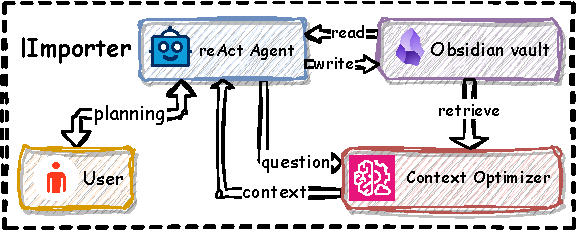
\includegraphics[width=0.85\textwidth]{figures/limporter.pdf}
    \caption{Esquema general del flujo de trabajo del agente lImporter.}
    \label{fig:importer_schema}
\end{figure}

Para la implementación de \textit{lImporter}, se propone un agente autónomo basado en el paradigma \textit{ReAct (Reasoning and Acting)}. Este agente está dotado de un conjunto de herramientas especializadas que le permiten interactuar directamente con la bóveda de \textit{Obsidian}, leyendo su estructura, obteniendo el contenido de las notas y escribiendo nueva información.

La explicación de la arquitectura se realizará de manera \textit{top-down}. Se comenzará describiendo el entorno y el funcionamiento general del agente, para luego profundizar en cada uno de sus componentes clave: el mecanismo de interacción con la bóveda y las estrategias para la obtención de contexto relevante.

\section{Descripción del entorno}
El entorno de trabajo para este proyecto es \textit{Obsidian}. A diferencia de otras herramientas basadas en la nube, el modelo de datos de \textit{Obsidian} es simple y robusto: una carpeta local en el sistema de archivos del usuario que contiene todos los datos. Las notas se almacenan como archivos de texto plano en formato \textit{Markdown} (`.md`), y pueden organizarse en una jerarquía de carpetas tradicional. Este enfoque garantiza la portabilidad, la longevidad y el control total del usuario sobre su información.

Una de las características más distintivas de \textit{Obsidian} es su capacidad para visualizar las conexiones entre notas como un grafo de conocimiento. Cada nota es un nodo en el grafo, y los vínculos entre notas se representan como aristas. Esto permite al usuario descubrir relaciones emergentes y navegar por su conocimiento de una manera no lineal. El grafo de \textit{Obsidian} es un \textbf{grafo dirigido por fuerzas} (\textit{force-directed graph}), una simulación física donde los nodos se repelen entre sí, mientras que los enlaces actúan como resortes que los atraen. Este mecanismo provoca que los nodos con conexiones en común, incluso indirectas, se agrupen visualmente, revelando clústeres temáticos de forma intuitiva (ver Figura~\ref{fig:obsidian_force_graph_example}).

\begin{figure}[h]
    \centering
    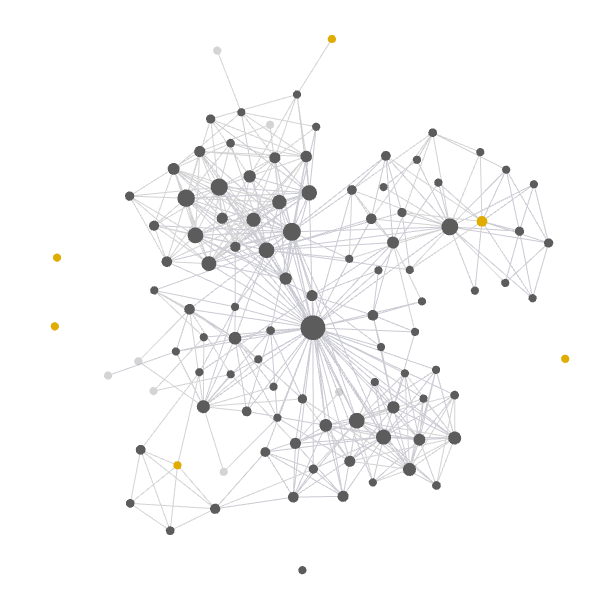
\includegraphics[width=0.66\textwidth]{figures/obsidian_kg_example.png}
    \caption{Ejemplo de la vista de grafo en Obsidian, mostrando nodos y sus interconexiones.}
    \label{fig:obsidian_graph}
\end{figure}

La creación de vínculos es fundamental para construir el grafo. En \textit{Obsidian}, esto se logra mediante la sintaxis de \textit{wikilinks}, simplemente encerrando el nombre de otra nota entre dobles corchetes, por ejemplo, `[[Nota Destino]]`. Además de los vínculos simples, \textit{Obsidian} soporta la \textbf{transclusión}, que permite incrustar el contenido de una nota (o una sección de ella) dentro de otra usando la sintaxis `![[Nota a Incrustar]]`. En la estructura del grafo, tanto un vínculo simple `[[...]]` como una transclusión `![[...]]` crean una conexión directa y equivalente entre los nodos correspondientes, contribuyendo por igual a la dinámica de fuerzas. La transclusión, por tanto, enriquece el contenido de la nota sin alterar la naturaleza del vínculo en el grafo.

\begin{figure}[h!]
    \centering
    \begin{subfigure}[b]{0.48\textwidth}
        \centering
        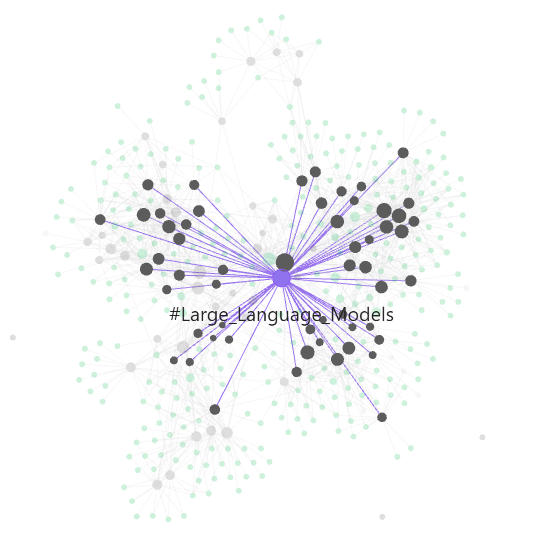
\includegraphics[width=\textwidth]{figures/LLM_tag_graph.png}
        % \caption{Vista del grafo centrada en la etiqueta \#Large Language Models.}
        \label{fig:llm_tag}
    \end{subfigure}
    \hfill
    \begin{subfigure}[b]{0.48\textwidth}
        \centering
        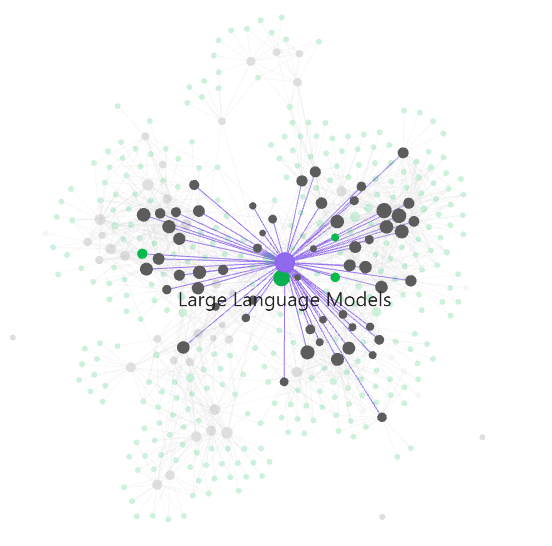
\includegraphics[width=\textwidth]{figures/LLM_note_graph.png}
        % \caption{Vista del grafo centrada en la nota Large Language Models.md.}
        \label{fig:llm_note}
    \end{subfigure}
    \caption{Comparación de la vecindad de la etiqueta \texttt{\#Large\_Language\_Models} y la nota \texttt{Large\_Language\_Models.md}.}
    \label{fig:obsidian_force_graph_example}
    \note{La proximidad visual entre el nodo de la etiqueta (izquierda) y el nodo de la nota (derecha) es un efecto directo del diseño basado en fuerzas. Al estar ambos conectados a un conjunto casi idéntico de notas, son atraídos hacia sus vecinos comunes, lo que resulta en su agrupación natural dentro del grafo.}
\end{figure}

\section{Agente \textit{reAct}}
En el núcleo del sistema se encuentra un agente basado en el \textit{framework ReAct} \parencite{yaoReActSynergizingReasoning2023}. Este paradigma permite a los modelos de lenguaje combinar el razonamiento (\textit{thought}) con la acción (\textit{action}). El agente opera en un ciclo donde, a partir de una tarea y una observación del entorno, razona sobre el siguiente paso a seguir, elige una herramienta de su repertorio, la ejecuta, y observa el resultado para informar su siguiente ciclo de razonamiento.

Siguiendo las mejores prácticas observadas en agentes avanzados como los utilizados para investigación o codificación (e.g. \textit{Deep Research}), se ha adoptado la estrategia \textit{Plan-and-Solve} \parencite{wangPlanandSolvePromptingImproving2023}. En lugar de actuar de forma impulsiva, el agente primero genera un plan detallado y paso a paso para resolver la tarea. El usuario tiene la opción de revisar, confirmar y dar retroalimentación sobre el plan generado antes de su ejecución. Este enfoque de \textit{human-in-the-loop} combina la eficiencia del planeamiento autónomo con la supervisión y el direccionamiento estratégico del usuario.

Para la implementación del agente se utiliza la familia de modelos \textit{Gemini} de \textit{Google}, debido a su multi-modalidad nativa, accesibilidad y, de manera crucial, su soporte nativo para \textit{function calling}, un mecanismo que se detallará a continuación.

\subsection{Interacción con la bóveda}
La capacidad del agente para leer y escribir archivos en la bóveda es posible gracias al uso de la \textit{API} de \textit{Obsidian}, orquestada a través de \textit{Function Calling}. Esta técnica puede ser entendida como un caso particular de \textit{style prompting} que emplea decodificación restringida (\textit{constrained decoding}) para forzar al modelo de lenguaje a generar una salida que se adhiere estrictamente a una gramática o formato predefinido \parencite{gengGrammarConstrainedDecodingStructured2024}.

En el caso de la \textit{API} de \textit{Gemini}, esta restricción obliga al modelo a producir una salida en formato \textit{JSON} que se corresponde con la firma de una de las funciones (herramientas) disponibles. Se aprovecha esta capacidad para mejorar la fiabilidad del agente. Por ejemplo, al definir los parámetros de una función, se puede utilizar el tipo de dato `\textit{ENUM}` para restringir las entradas a un conjunto de valores válidos (e.g., una lista de carpetas o archivos existentes), evitando así que el modelo intente operar sobre rutas inválidas o alucinadas.

\subsubsection{Lectura}
Para la lectura de información de la bóveda, el agente dispone de dos herramientas principales:
\begin{itemize}
    \item \texttt{tree(path)}: Esta función recibe la ruta a una carpeta raíz y devuelve una representación textual de la estructura de directorios y archivos contenida en ella, de forma análoga al comando \texttt{tree} de la línea de comandos. Esto permite al agente obtener una visión global de la organización de la bóveda.
    \item \texttt{read(path)}: Esta función recibe la ruta a un archivo \textit{Markdown} (`.md`) existente y devuelve su contenido completo como texto.
\end{itemize}
 
\subsubsection{Escritura}
Un desafío común en los agentes que interactúan con sistemas de archivos es la tendencia del modelo a generar rutas de archivo incorrectas o con nombres similares pero no idénticos a los existentes. Para mitigar este problema, la capacidad de escritura se ha separado en dos funciones distintas:
\begin{itemize}
    \item \texttt{mkdir(path)}: Permite al agente crear un nuevo directorio en una ubicación específica de la bóveda, asegurando que la estructura de carpetas deseada exista antes de intentar escribir un archivo.
    \item \texttt{write(path, content)}: Crea un nuevo archivo o sobrescribe el contenido de uno existente. El parámetro \texttt{path} de esta función se beneficia directamente de la decodificación restringida, ya que se puede guiar al modelo para que elija entre rutas sugeridas o siga un formato válido, reduciendo drásticamente los errores.
\end{itemize}
 
\subsubsection{Obtencion de contexto}
Para que el agente pueda tomar decisiones informadas, como determinar dónde crear una nueva nota o con qué notas existentes vincularla, necesita un contexto relevante de la bóveda. Dado que el contenido total de la bóveda puede exceder fácilmente la ventana de contexto del modelo, se utiliza un enfoque de divide y vencerás.

Se propone una función que recibe un conjunto de archivos y un límite de tokens. Si el contenido combinado de los archivos excede el límite, el conjunto se divide recursivamente por la mitad hasta que los fragmentos resultantes son lo suficientemente pequeños. Una vez que un fragmento cabe en la ventana de contexto, un modelo de lenguaje se encarga de extraer la información relevante de él. La naturaleza de esta información relevante se define por un nivel de \textbf{granularidad} especificado por el usuario (en \cite{chenDenseRetrievalWhat2024} se analiza la optimalidad de selección de diferentes casos de estos).

Esta idea está inspirada en la técnica propuesta en \cite{shenQwenLongCPRS$infty$LLMsDynamic2025}. De manera similar, se proponen tres niveles de granularidad:
\begin{itemize}
    \item \textbf{Paragraph}: Ideal para obtener resúmenes y el sentido general de un documento.
    \item \textbf{Sentence}: Extremadamente útil para identificar afirmaciones específicas y recuperar relaciones entre conceptos.
    \item \textbf{Keyword}: Perfecto para la extracción de entidades nombradas y conceptos clave.
\end{itemize}

A continuación se presenta un pseudocódigo del proceso de obtención de contexto:

\begin{verbatim}
function getContext(files, token_limit, granularity):
    if total_tokens(files) <= token_limit:
        return extract_info(files, granularity)
    else:
        mid = floor(len(files) / 2)
        part1 = files[0:mid]
        part2 = files[mid:len(files)]
        
        context1 = getContext(part1, token_limit, granularity)
        context2 = getContext(part2, token_limit, granularity)
        
        return combine(context1, context2)
\end{verbatim}

\subsection{Sobre la versatibilidad del sistema}
Un objetivo clave de \textit{lImporter} es su versatilidad para integrarse en diversos flujos de trabajo. El agente debe ser útil tanto para un usuario que desea construir una base de conocimiento densamente interconectada, generando múltiples relaciones y resúmenes, como para otro que simplemente quiere archivar un nuevo concepto de forma aislada, sin crear ningún vínculo.

La arquitectura basada en un agente \textit{ReAct} y el sistema de obtención de contexto granular sustentan esta flexibilidad. El agente puede recibir instrucciones para ser exhaustivo en la búsqueda de conexiones o, por el contrario, para limitarse a crear una nota y guardarla en una carpeta específica. Sin embargo, esta versatilidad conlleva un incremento en la labor manual de configuración inicial, ya que el comportamiento del agente se define en gran medida a través de un archivo de instrucciones proporcionado por el usuario.

\chapter{Experimentos}\label{chapter:implementation}
En este capítulo se presentan una serie de experimentos diseñados para evaluar el rendimiento y las capacidades del agente \textit{lImporter}. Es importante aclarar que no se realizó un análisis holístico y cuantitativo del sistema. En su lugar, se optó por explorar distintos casos de uso que demuestran la versatilidad de la herramienta y ponen de manifiesto las interesantes posibilidades que surgen al integrar un agente de lenguaje autónomo en una bóveda de conocimiento de Obsidian.

\section{Base estructurada sobre \textit{Harry Potter}}
En el primer experimento, se utilizó la versatilidad del agente para una tarea clásica: la creación de una base de conocimientos estructurada sobre el universo de \textit{Harry Potter}. El objetivo era proporcionar al agente el \textit{PDF} del primer libro y pedirle que generara notas para personajes, lugares y conceptos clave, vinculándolos entre sí. Este caso de uso potencia a Obsidian como una herramienta para la exploración visual del conocimiento a través de su vista de grafo.

Es relevante mencionar que, por defecto, Obsidian no muestra etiquetas en las aristas del grafo, lo que dificulta la interpretación de la naturaleza de las relaciones. Para solventar esto, se utilizó un plugin llamado \textit{Graph Link Types} de la comunidad que añade dicha funcionalidad. El grafo resultante, como se muestra en la Figura \ref{fig:hp_graph}, fue creado exitosamente. 

\begin{figure}[h]
    \centering
    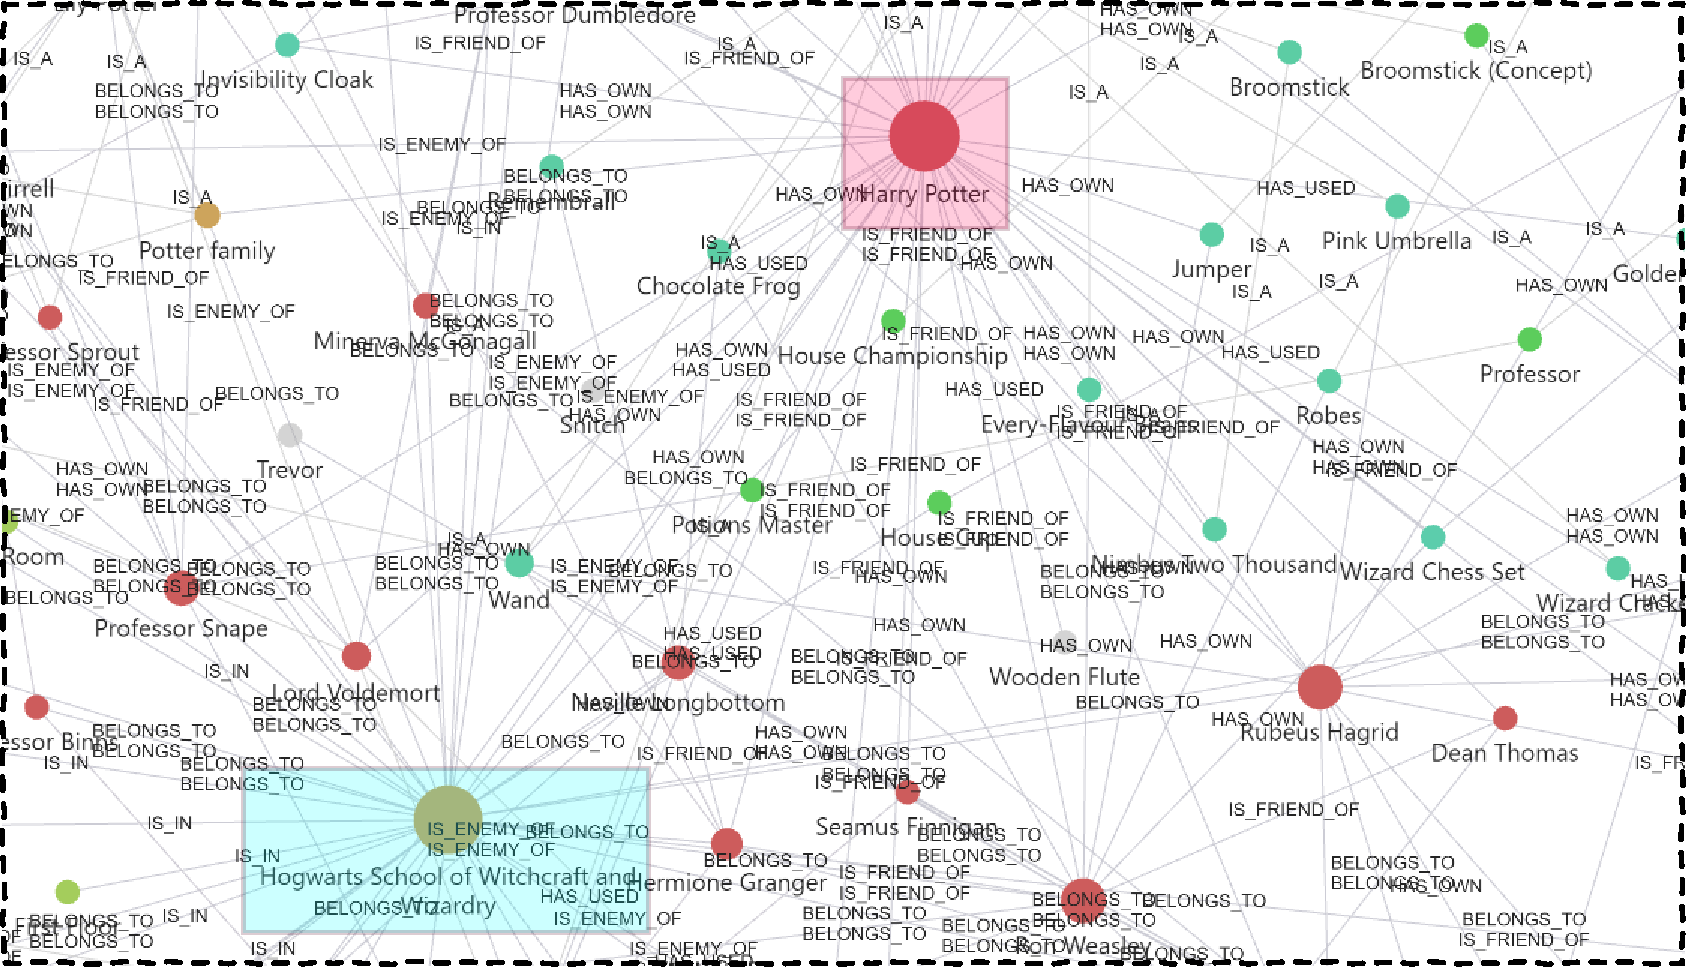
\includegraphics[width=1.0\textwidth]{figures/HPKG.pdf}
    % \fbox{\parbox[c][15em][c]{0.8\textwidth}{\centering \huge Placeholder: \\ Grafo de conocimiento de Harry Potter generado por el agente}}
    \caption{Grafo resultante del experimento de \textit{Harry Potter}, mostrando la centralidad de nodos clave.}
    \label{fig:hp_graph}
\note{En la figura, se observa que conceptos centrales como \textit{Harry Potter} (resaltado en rojo) y \textit{Hogwarts} (en azul) se representan con nodos de mayor tamaño. Esto se debe a que \textit{Obsidian} modula el tamaño de cada nodo en función de su grado —el número de conexiones que posee—, lo que resalta visualmente la importancia de las entidades más conectadas y demuestra la utilidad de esta representación incluso para bases de conocimiento ya estructuradas.}
\end{figure}

Es importante señalar que este experimento no fue diseñado con el objetivo de realizar una extracción de entidades exhaustiva y precisa. Su propósito principal era demostrar la capacidad del sistema para abordar un caso de uso estructurado con la configuración adecuada. Aun así, los resultados evidencian cómo el agente puede generar rápidamente una representación del conocimiento que es tanto visualmente atractiva como funcional, constituyendo un excelente punto de partida para el análisis preliminar de cualquier dominio.

\section{Añadiendo artículos a una \textit{Wiki} tecnológica}
Este experimento se diseñó para simular el mantenimiento y crecimiento de una base de conocimiento existente. Se partió de una bóveda de \textit{Obsidian} que funcionaba como una \textit{wiki} personal sobre temas de tecnología (programación, \textit{hardware/software}, etc.). Progresivamente, se le proporcionaron al agente nuevos archivos, acompañados de un breve audio con instrucciones.

\begin{figure}[h!]
    \centering
    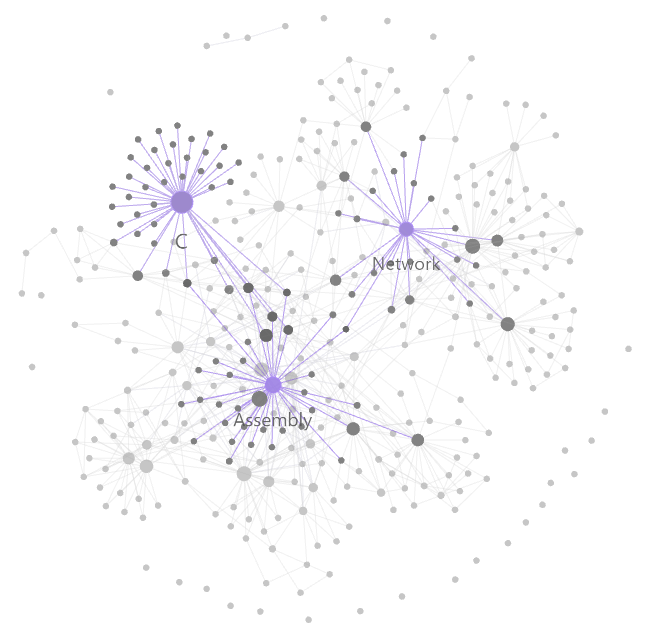
\includegraphics[width=0.6\textwidth]{figures/WikiSamples2.png}
    \caption{\textit{Wiki} personal sobre temas de tecnología.}
    \label{fig:wiki_tech_graph}
\end{figure}

El objetivo era doble. Por un lado, se buscaba demostrar que el agente es capaz de analizar el nuevo contenido, comprenderlo en el contexto de la bóveda existente y determinar correctamente con qué notas preexistentes debía vincularlo. Por otro lado, y de igual importancia, se quería verificar que el agente no siempre establece conexiones. Si un nuevo artículo trata sobre un tema completamente ajeno a lo que ya existe en la bóveda, el resultado deseable es que se cree una nota aislada, sin vínculos forzados o incorrectos. Este comportamiento es crucial para mantener la integridad y la calidad del grafo de conocimiento.

Para evaluar estos comportamientos, se realizaron dos secuencias de inserción. En la primera, se introdujeron artículos sobre hardware neuromórfico y alternativas a \textit{backpropagation}, temas sin representación previa en la bóveda. Como se esperaba, el agente creó las notas correspondientes pero no las vinculó con el grafo existente (Figura \ref{fig:wiki_isolated}). En la segunda secuencia, se añadió una serie de artículos sobre los orígenes de las \textit{Interaction Nets} y sus aplicaciones actuales, un tema con precursores ya presentes en la \textit{wiki}. En este caso, el agente sí estableció las conexiones pertinentes, integrando los nuevos nodos con el conocimiento previo (Figura \ref{fig:wiki_connected}).

\begin{figure}[h!]
    \centering
    \begin{subfigure}[b]{0.48\textwidth}
        \centering
        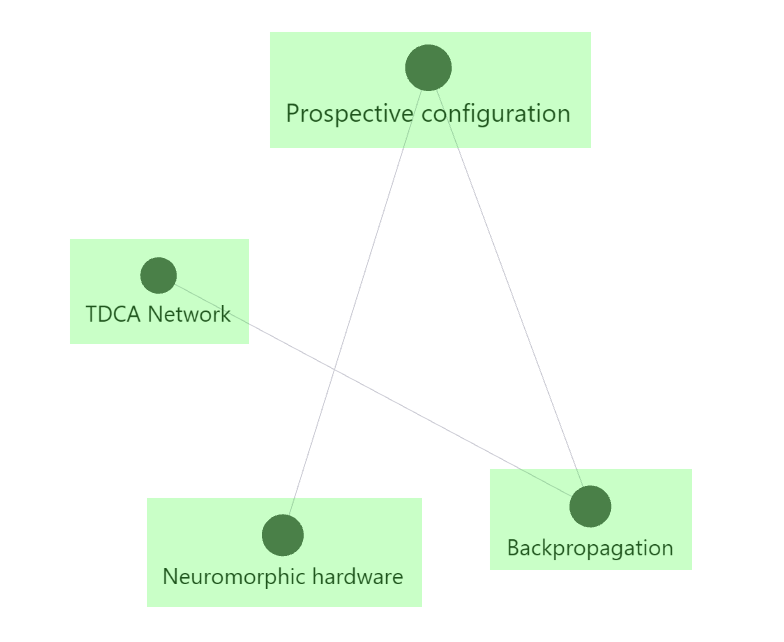
\includegraphics[width=\textwidth]{figures/neuromPart.png}
        % \fbox{\parbox[c][12em][c]{0.9\textwidth}{\centering \huge Placeholder: \\ Grafo de nodo aislado}}
        \caption{Notas sobre hardware neuromórfico sin conexiones externas a las nuevas.}
        \label{fig:wiki_isolated}
    \end{subfigure}
    \hfill
    \begin{subfigure}[b]{0.5\textwidth}
        \centering
        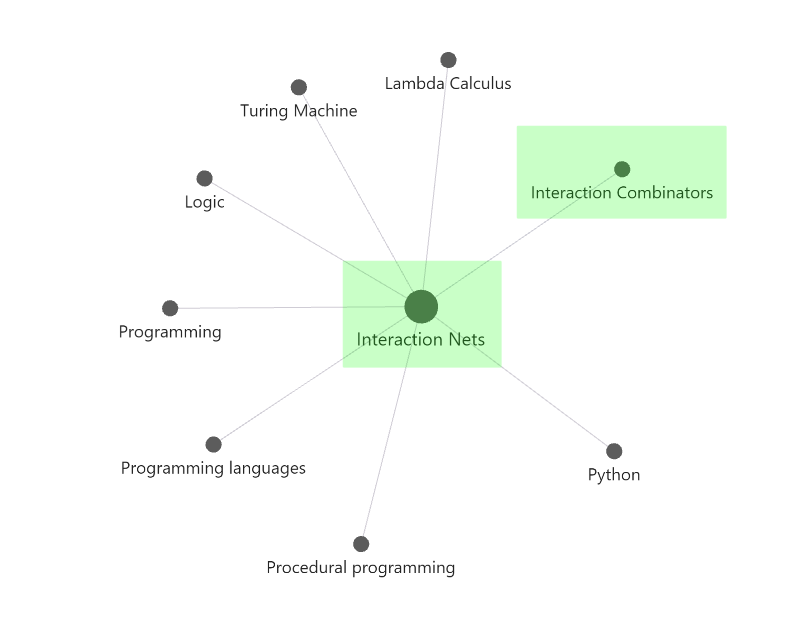
\includegraphics[width=\textwidth]{figures/IntNetsPart.png}
        % \fbox{\parbox[c][12em][c]{0.9\textwidth}{\centering \huge Placeholder: \\ Grafo local conectado}}
        \caption{Notas sobre \textit{Interaction Nets} conectadas a notas existentes.}
        \label{fig:wiki_connected}
    \end{subfigure}
    \caption{Comparación de resultados de inserción con las notas nuevas resaltadas.}
    \label{fig:wiki_comparison}
\note{Ambas vistas corresponden al grafo local de Obsidian. En el caso aislado (izquierda), se muestra con profundidad máxima (5), pero al no tener vínculos, solo aparecen los nodos resultantes de la secuencia de inserción. En el caso conectado (derecha), una profundidad de 1 es suficiente para visualizar las conexiones a notas existentes.}
\end{figure}

En conjunto, estos resultados verifican la versatilidad del agente para determinar, de forma autónoma, qué notas existentes son candidatas idóneas para establecer vínculos con el nuevo contenido. Esta capacidad de discernimiento, reforzada por el optimizador de contexto, es fundamental para asegurar que la base de conocimiento crezca de manera coherente y relevante.

\section{Projects, Areas, Resources, Archived}
Este experimento refleja un caso de uso más cotidiano y de productividad personal, siguiendo la metodología \textit{P.A.R.A}. \textit{(Projects, Areas, Resources, Archived)} popularizada por \cite{forteBuildingSecondBrain2022}. El objetivo era evaluar si el sistema puede ser utilizado para mantener una bóveda organizada bajo esta estructura, siguiendo instrucciones de voz. Para ello, se realizaron experimentos donde cada petición consistía en un archivo de audio, acompañado opcionalmente por archivos de contexto adicionales.

Se evaluó la capacidad del modelo para realizar diversas tareas, entre las que destacan:
\begin{itemize}
    \item \textbf{Agregar detalles a proyectos existentes:} Por ejemplo, se solicitó añadir una nueva canción al proyecto de práctica de canto, proporcionando como contexto un documento con la letra adicional al audio con la instrucción.
    \item \textbf{Reescribir y sintetizar información:} Se instruyó por voz al modelo para que buscara información dispersa sobre un proyecto de tesis dentro de la bóveda. El contenido encontrado fue sintetizado en un nuevo documento. Además se propusieron nuevas ideas para complementar el trabajo en un documento adicional.
    \item \textbf{Crear nuevos proyectos:} Se crearon proyectos desde cero con indicaciones sobre sus objetivos y se vincularon a otros existentes. Por ejemplo, se generó un 'Nuevo proyecto de proyección vocal' vinculado al proyecto de 'práctica de canto'.
\end{itemize}

Adicionalmente, este experimento contaba con instrucciones para la automatización de flujos. El agente no solo procesaba la petición, sino que también extraía la transcripción a un nuevo archivo y organizaba los ficheros procesados, probando así sus capacidades para automatizar tareas. Incluir los archivos generados en este documento sería verboso y no aportaría más información que la confirmación de que fueron creados correctamente. Por ello, los resultados y los nuevos ficheros se pueden consultar en el repositorio del proyecto.

\section{\textit{Note augmented LLMs are computationally universal}}
Este último experimento, de naturaleza más teórica, se inspira en la idea de que los modelos de lenguaje, cuando se aumentan con una memoria externa, pueden volverse computacionalmente universales \parencite{schuurmansMemoryAugmentedLarge2023}.

Para explorar esta idea, se le pidió al agente que evaluara la Conjetura de Collatz para un número dado, utilizando una nota de \textit{Obsidian} como su \textit{memoria de trabajo} o registro. En cada paso de la secuencia, el agente leía el estado actual de la nota, calculaba el siguiente número, y sobrescribía la nota con el nuevo valor.

\begin{figure}[h]
    \centering
    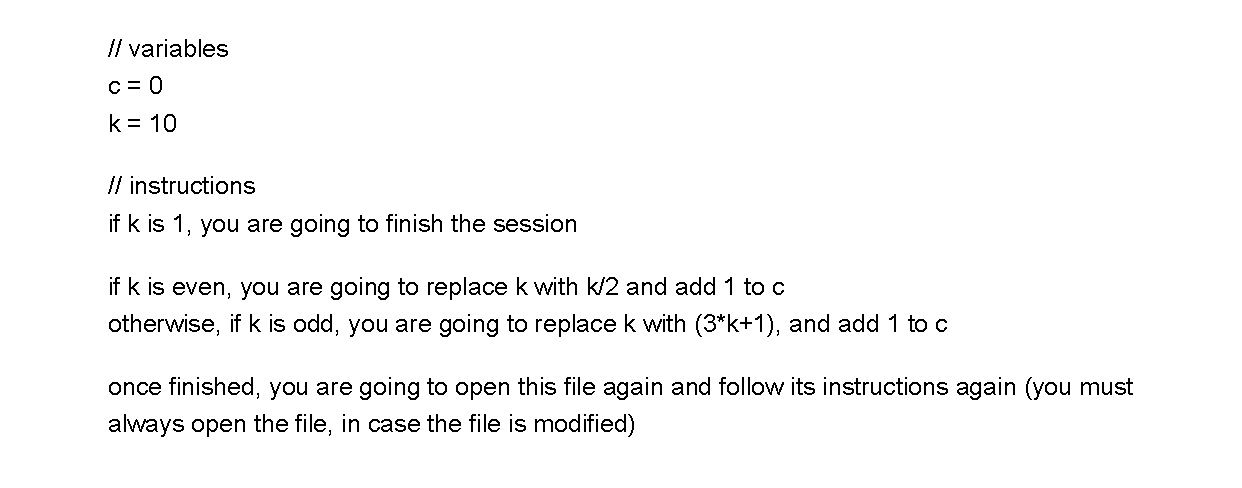
\includegraphics[width=1.0\textwidth]{figures/collatz_init_10.pdf}
    % \fbox{\parbox[c][15em][c]{0.45\textwidth}{\centering \huge Placeholder: \\ Contenido de la nota de Collatz}}
    \caption{Contenido inicial de la nota de trabajo para $n=10$ en la evaluación de Collatz.}
    \label{fig:collatz_code}
\end{figure}

Se evaluó el caso para $n=10$, que se resolvió correctamente en 6 iteraciones (Figuras \ref{fig:collatz_code} y \ref{fig:collatz_diff}). También se evaluaron casos más largos como $n=11$ (14 iteraciones) y $n=27$ (111 iteraciones). Este último caso excedió los límites de cuota de la API y requirió reiniciar el proceso, lo cual demostró una capacidad emergente del sistema: la posibilidad de dejar una tarea y seguirla luego, ya que el estado se preserva en la nota de \textit{Obsidian}.

La intuición subyacente es que la capacidad de releer el estado desde un archivo fiable reduce drásticamente la probabilidad de error en un proceso iterativo largo, de manera análoga a cómo una \textit{CPU} depende de leer y escribir correctamente en sus registros. En este caso se usó un modelo potente en razonamiento algebraico (\textit{Gemini 2.5 Flash}). Si bien un modelo más modesto podría fallar en esta tarea matemática, la misma arquitectura podría permitirle automatizar con alta fiabilidad otra tarea iterativa que se alinee con sus fortalezas (por ejemplo, un análisis de sentimiento refinado a lo largo de múltiples revisiones), siempre que sea proficiente en las operaciones básicas de leer y escribir en su memoria externa.

\begin{figure}[h]
    \centering
    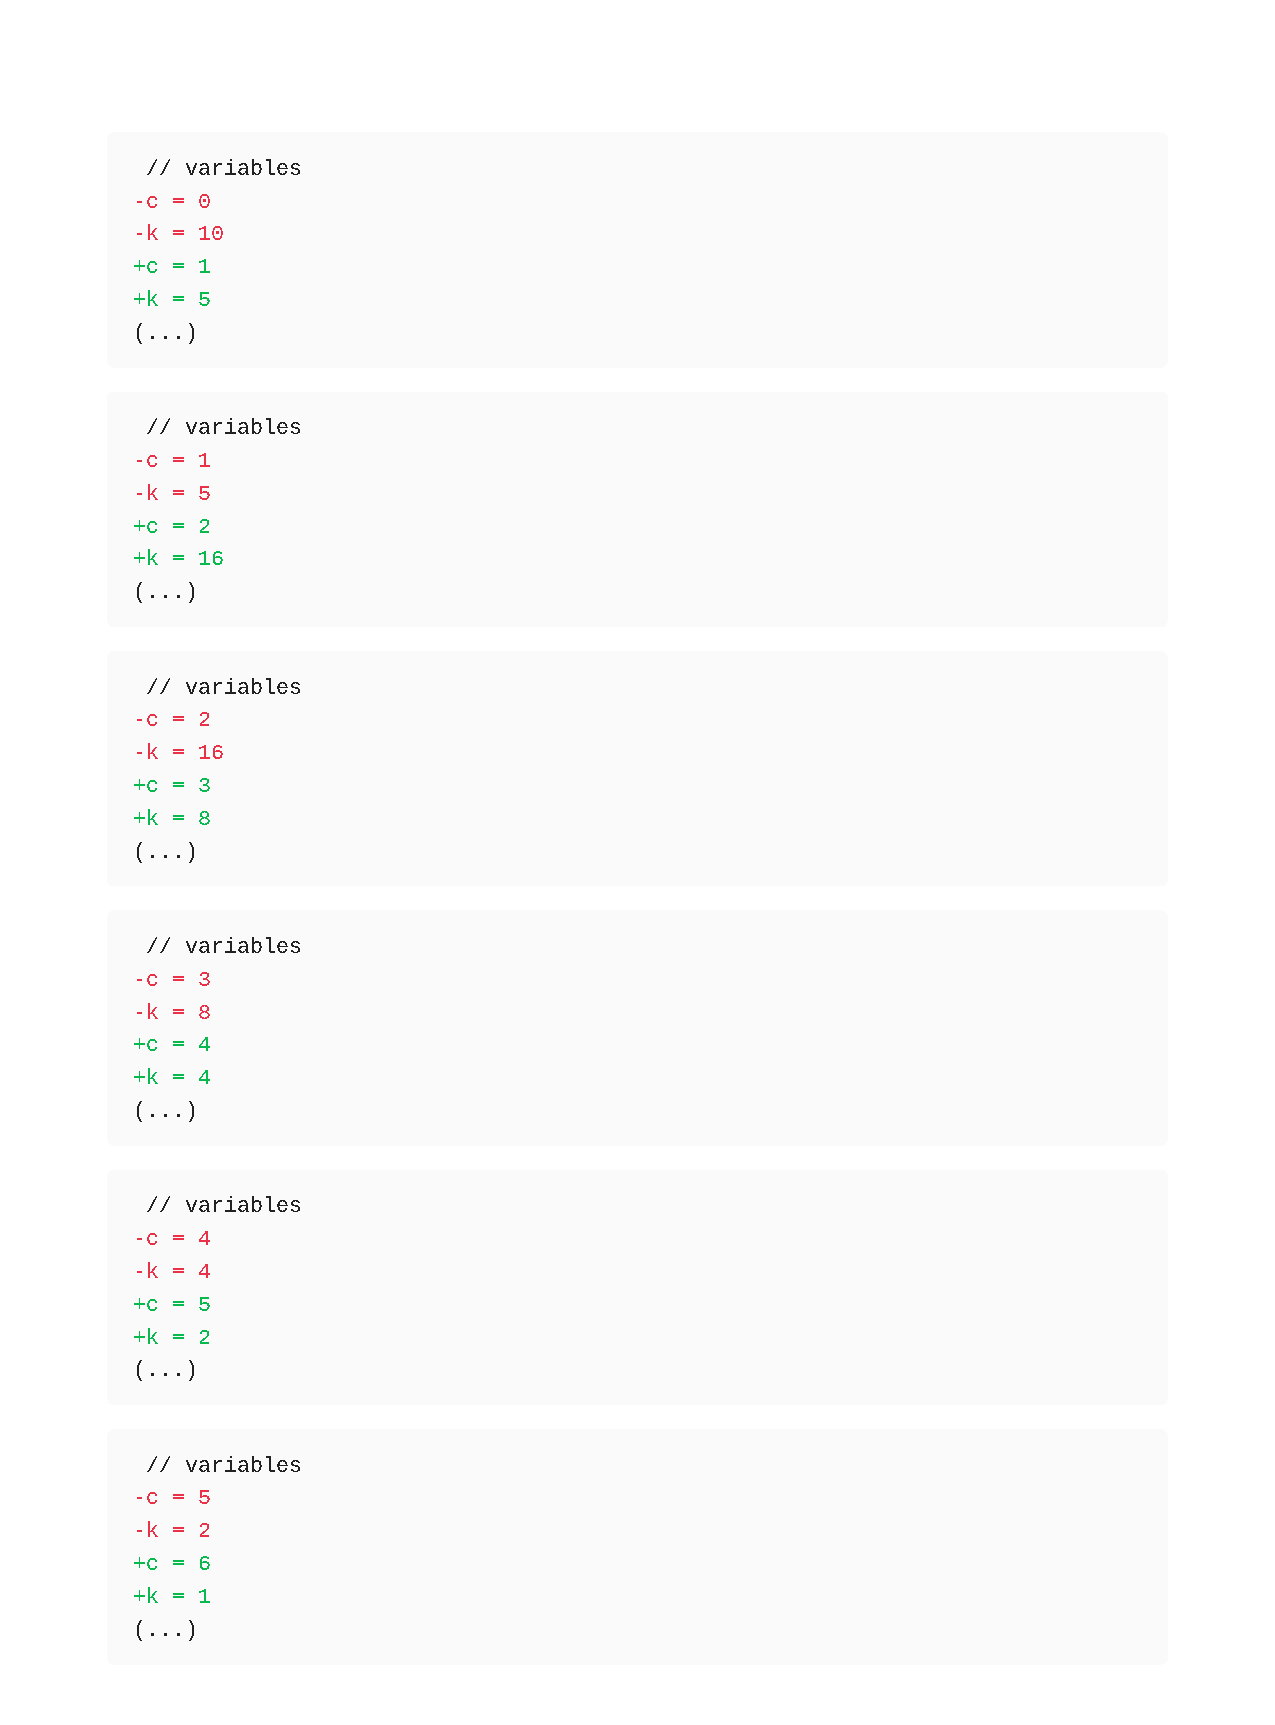
\includegraphics[width=1.0\textwidth]{figures/clltz_logs_10.pdf}
    % \fbox{\parbox[c][15em][c]{0.45\textwidth}{\centering \huge Placeholder: \\ Diff entre iteraciones}}
    \caption{Diferencia en el contenido de la nota entre los pasos de la evaluación para $n=10$.}
    \label{fig:collatz_diff}
\end{figure}
%\chapter*{Conclusiones}
\addcontentsline{toc}{chapter}{Conclusiones}

El presente trabajo de tesis se propuso abordar el desafío de optimizar la integración de conocimiento en bases personales semiestructuradas, un proceso tradicionalmente manual y laborioso. La investigación partió de la pregunta de si un agente personalizable basado en Grandes Modelos de Lenguaje (\textit{LLM}) podría automatizar y enriquecer este proceso de manera eficaz y adaptable a diversos paradigmas de toma de notas. La respuesta, materializada en el prototipo \textbf{lImporter}, es afirmativa y abre la puerta a una nueva generación de herramientas para la Gestión del Conocimiento Personal (PKM).

Se cumplieron los objetivos específicos planteados al inicio de la investigación. Primero, se desarrolló un \textit{framework} flexible en forma del \textit{plugin} `lImporter` para \textit{Obsidian.md}, capaz de procesar diversas fuentes de información. Segundo, se diseñó e implementó un agente autónomo basado en el paradigma \textit{ReAct}, cuya arquitectura combina la estrategia \textit{Plan-and-Solve} con la interacción fiable mediante \textit{function calling}, y un innovador sistema de optimización de contexto para consultar eficientemente la bóveda del usuario. Finalmente, la evaluación, realizada a través de una serie de experimentos cualitativos, demostró la versatilidad y eficacia del sistema para cumplir con los requisitos de distintos flujos de trabajo.

Los experimentos revelaron capacidades clave y matices importantes del sistema. La creación de una base de conocimiento sobre Harry Potter demostró la habilidad del agente para construir grafos de conocimiento estructurados y visualmente funcionales a partir de texto no estructurado. El mantenimiento de una wiki tecnológica evidenció una capacidad crucial: el discernimiento para crear conexiones relevantes cuando existen, y para mantener aislados los conceptos nuevos y no relacionados, preservando así la integridad del conocimiento. El experimento con la metodología P.A.R.A. validó su utilidad en escenarios de productividad personal más dinámicos y cotidianos. Por último, el experimento teórico de la Conjetura de Collatz desveló una capacidad emergente y profunda: la posibilidad de utilizar la base de notas como una memoria externa fiable, permitiendo al \textit{LLM} realizar tareas iterativas y con estado de una manera robusta, análoga a un ciclo de computación.

A pesar de los resultados positivos, el trabajo presenta limitaciones inherentes. La calidad de las acciones del agente está intrínsecamente ligada a la capacidad de razonamiento del \textit{LLM} subyacente. Asimismo, la dependencia de APIs externas implica costos monetarios y límites de uso que pueden restringir la ejecución de tareas muy extensas. La versatilidad del sistema, si bien es una fortaleza, también introduce una dependencia de la habilidad del usuario para formular instrucciones claras y efectivas (\textit{prompting}). Finalmente, la evaluación fue de naturaleza cualitativa, centrándose en demostrar la viabilidad y el potencial, en lugar de realizar una comparativa cuantitativa rigurosa.

Las futuras líneas de investigación pueden expandir este trabajo en varias direcciones. La integración de modelos de lenguaje de código abierto y de ejecución local podría mitigar los costos y las preocupaciones de privacidad. Sería valioso dotar al agente de la capacidad de interactuar con otras herramientas y \textit{plugins} del ecosistema de \textit{Obsidian}, como \textit{Dataview}, para realizar consultas estructuradas sobre la base de conocimiento. Se podría explorar el desarrollo de agentes proactivos que operen en segundo plano, sugiriendo conexiones o reorganizaciones sin una petición explícita del usuario. La evolución hacia sistemas multi-agente, donde diferentes agentes especializados colaboran en tareas complejas, representa una frontera prometedora.

En conclusión, este trabajo demuestra que la sinergia entre los \textit{LLM} y los sistemas de PKM va más allá de la simple asistencia conversacional. Al dotar a los modelos de lenguaje de un cuerpo de conocimiento externo y la capacidad de actuar sobre él, se transforman en verdaderos colaboradores cognitivos. \textbf{lImporter} se erige como un prototipo funcional que valida este paradigma, mostrando un camino viable hacia la construcción de un "segundo cerebro" que no solo almacena información, sino que activamente ayuda a estructurarla, conectarla y generar nuevas ideas a partir de ella.

% ===== BIBLIOGRAPHY =====
\cleardoublepage{}
\phantomsection{}
\addcontentsline{toc}{chapter}{\bibname}
\printbibliography{}

% \thispagestyle{empty}% % No page number on bib

\end{document}